\section{Systematic uncertainties}
\label{sect:sys}
Systematic uncertainties can affect the shape or normalization of the
backgrounds estimated from Monte Carlo (\ttbar, $Z+$ jets, dibosons and Higgs decays and \wjets in \tauTau \bintwo), 
as well as the signal acceptance. 
\subsection{Luminosity}
The uncertainty on the luminosity  is $2.6\%$ for $2012$ data ~\cite{LUMI}.

\subsection{b-jet veto uncertainty due to mismodelling of ISR}
The jet activity in our signal is just due to Initial State Radiation(ISR). The ISR is not simulated properly in our signal, because it has been generated using \PYTHIA $6.4$ event generator and it just produces $2 \rightarrow 2$ scattering processes. Therefore the ISR jet momenta spectra and its multiplicity cannot be trusted. It is possible that an ISR jet is mistagged as a b-jet and results in vetoing the signal event after applying the b-veto cut. On the other side \MADGRAPH ~\cite{MADGRAPH} generator, which is a matrix element generator provides a better description of ISR jets by supporting $2 \rightarrow 4$ interactions. To measure the amount of uncertainty introduced by b-veto cut we can compare the efficiency of this cut in our generated signal and its value in a sample similar to our signal which has been generated by \MADGRAPH. 
The most similar MC sample to our signal from the production point of view is WW sample. The $m(\chione) = 100\,\GeV$ and $m(\PSGczDo) = 1\,\GeV$ point of the signal is chosen so that masses resembles the WW production mechanism. % It is followed the below recipe, originating from $fixME$.
%By applying and relaxing the b-veto cut it is obtained the yields of WW and signal and by the uncertainty is A:
We obtain the efficiency of b-veto for signal sample denoted as $E^{SUSY}_{b-veto}$ and also for WW sample denoted as $E^{WW}_{b-veto}$.
Comparing these 2 efficiencies this uncertainty can be estimated.

%\begin{linenomath}
%\begin{equation}
%\label{eq:suWW}
%I_{e/ \mu}=\Sigma P_{T}^{charged }(\Delta z <2mm)+max(P_{T}^{photon}+P_{T}^{h0 }-\Delta \beta,0),

\begin{align}
E^{WW}_{b-veto} &= \frac{WW_{0b}}{WW_{all}} = \frac{88968.51}{93058.33} = 0.95\\ \nonumber
\end{align}
and the b-veto efficiency for the signal is:
\begin{align}
E^{SUSY}_{b-veto} &= \frac{SUSY_{0b}}{SUSY_{all}} = \frac{2041.88}{2206.07} = 0.92 \\ \nonumber
\end{align}
and we take:
\begin{align}
|\frac{E^{SUSY}_{b-veto}-E^{WW}_{b-veto}}{E^{WW}_{b-veto}}| &= 3 \% \\ \nonumber
\end{align}

%\end{equation}
%\end{linenomath}

%The differences between MC and data should be considered as another source of systematics too. As the efficiency of selecting WW events in data is too low, the effect of b-veto scale factors is measured as an upper limit.

%\begin{linenomath}
%\begin{align}
%\label{eq:suWW}
%I\_{e/ \mu}=\Sigma P\_{T}^{charged }(\Delta z <2mm)+max(P\_{T}^{photon}+P\_{T}^{h0 }\_\Delta \beta,0),
%E^{data}_{b-veto} &= \frac{data\_b-veto applied}{data\_b-veto relaxed} = \frac{80282.30}{84226.93} = 0.956 \\ \nonumber
%\end{align}
%and we have:

% &= \frac{data\_ratio - WW\_ratio}{WW\_ratio} = 0.003 \% \nonumber

%\end{linenomath}

%The total uncertainty due to ISR systematic uncertainty is estimated as 3 \%.

\subsection{\texorpdfstring{Uncertainty due to $\mindphifour$ cut}{Uncertainty due to minDeltaPhiJMET cut}}
Another source of systematic uncertainty due to existence of ISR in signal events is the cut on $\mindphifour$ ($ > 1$) against QCD events. We use the same method as mentioned above to obtain the systematic uncertainty of applying this variable. But this time we use Higgs to $\tau \tau$ sample which mimics our signal most.
%and we chose it because Higgs sample has the most similar cumulative distribution function,i.e. the efficiency of this cut, to our signal that is shown in. %Fig.~\ref{}.     

\begin{align}
E^{Higgs}_{\mindphifour} &= \frac{Higgs_{\mindphifour>1.0}}{Higgs_{all}} = \frac{89288.14}{180562.56} = 0.49 \\ \nonumber
\end{align}
and this efficiency for the signal is: 
\begin{align}
E^{SUSY}_{\mindphifour} &= \frac{SUSY_{\mindphifour>1.0}}{SUSY_{all}} = \frac{1020.33}{2206.07} = 0.46 \\ \nonumber
\end{align}
and we take:
\begin{align}
|\frac{E^{SUSY}_{\mindphifour}-E^{Higgs}_{\mindphifour}}{E^{Higgs}_{\mindphifour}}| &= 6 \% \\ \nonumber
\end{align}

\subsection{\texorpdfstring{$\ell$ and $\hadtau$ energy scale}{Energy scale}}

The systematic uncertainty due to muon energy scale is small enough to be ignored.

The electron energy is varied by $1\%$ ($2.5\%$) for electrons reconstructed in the barrel (endcap) region as recommended by EGAMMA POG\cite{eEnergyScale}. As this variation has small effects on electron $\pt$ related variables, its effect on final yields in \eTau channel has been found negligible.

The energy of \hadtau's is scaled by $3\%$, following the recommendation of the Tau POG~\cite{TauPOG}. Variables like \MET, \mttwo, \mindphifour and invariant mass which depend on \hadtau $\pt$ are re-calculated.  Up and down uncertainties on the final yields are reported in table~\ref{Tab.tauEnergyScale}. In some cases which the statistical uncertainty had a large value comparing to systematic uncertainty, we relaxed some $\hadtau$ \pt  independent variables to obtain more statistics.

The big value of the \hadtau energy scale uncertainty is dominated by the lack of the statistics. In signal samples which have enough statistics the uncertainty decreases. So the maximum uncertainty due to \hadtau energy scale in MC driven backgrounds and signal is set to $~25\%$ and $~15\%$, respectively.
%In order to calculate systematic uncertainties for signal, we used 3 signal points which are ($m(\chione) = 180\,\GeV$, $m(\PSGczDo) = 60\,\GeV$), (240, 40) and (380, 1) representing low, moderate and high delta mass respectively. 
The $15\%$ effect of this uncertainty for all signal points in different channels is a conservative value that covers the whole plain and all channels.


%% \begin{table}[!h]
%% \tiny{
%% \begin{center}
%% \begin{tabular}{|c|c|c|c|c|c|c|c|c|}
%% \hline
%%                              & QCD & ZX    & W  & WW   & Top    & All MC & Susy & Data \\\hline 
%% $e\hadtau$ channel           & $0.0 ^{+0.0} _{-0.0} $ & $0.38 ^{+0.05} _{-0.03}  $    &  $1.2 ^{+0.0} _{-0.0} $      &  $0.05 ^{+0.0} _{-0.0} $   &$0.02 ^{+0.12} _{-0.0} $           & $1.74 ^{+0.13} _{-0.03} $       & $3.47 ^{+0.33} _{-0.0} $ & $3.0 ^{+0.0} _{-1.0}$    \\\hline   

%% $\mu\hadtau$ channel &  $0.0 ^{+0.0} _{-0.0} $     &  $0.28 ^{+0.11} _{-0.0} $      &  $0.79 ^{+0.0} _{-0.32} $  & $0.34 ^{+0.07} _{-0.05} $        &  $0.0 ^{+0.04} _{-0.06} $   &    $1.4 ^{+0.22} _{-0.34} $      &  $2.41 ^{+0.17} _{-0.02} $      & $5.0 ^{+1.0} _{-2.0} $     \\\hline  

%% $\tauTau$ channel bin1 &  $0.0 ^{+0.0} _{-0.0}$   &    $0.56 ^{+0.7} _{-0.09}$    &  $0.0 ^{+0.0} _{-0.0}$      &  $0.02 ^{+0.0} _{-0.02}$        &   $0.0 ^{+0.0} _{-0.0}$        &    $0.58 ^{+0.7} _{-0.11}$     & $4.1^{+0.24} _{-0.26} $    & $0.0 ^{+0.0} _{-0.0}$\\\hline

%% $\tauTau$ channel bin2 &  $0.0 ^{+0.0} _{-0.0}$   &     $0.81 ^{+0.39} _{-0.7}$     &    $0.43 ^{+0.0} _{-0.0}$     &     $0.15 ^{+0.1} _{-0.02}$     &   $0.53 ^{+0.0} _{-0.23}$   &      $1.91 ^{+0.28} _{-1.94}$     &     $3.13 ^{+0.12} _{-0.27}$   &  $0.0 ^{+0.0} _{-0.0}$    \\\hline
%% \end{tabular} 
%% \end{center}
%% \caption{Tau energy scale systematic effect on MC in different channels}
%% \label{Tab.susyHiggs}

%% }
%% \end{table}     

%% \begin{table}[!h]
%% \tiny{
%% \begin{center}
%% \begin{tabular}{|c|c|c|c|c|c|c|c|c|}
%% \hline
%%                              & QCD & ZX    & W  & WW   & Top    & All MC & Susy & Data \\\hline 
%% $e\hadtau$ channel           & $0.0 ^{+0.0 \%} _{-0.0 \%} $ & $0.38 ^{+13 \%} _{-5 \%}  $    &  $1.2 ^{+0.0 \%} _{-0.0 \%} $      &  $0.05 ^{+0.0 \%} _{-0.0 \%} $   &$0.02 ^{+600.0 \%} _{-0.0 \%} $           & $1.74 ^{+8 \%} _{-2 \%} $       & $3.47 ^{+9 \%} _{-0.0 \%} $ & $3.0 ^{+0.0 \%} _{-33 \%}$    \\\hline   

%% $\mu\hadtau$ channel &  $0.0 ^{+0.0 \%} _{-0.0 \%} $     &  $0.28 ^{+40 \%} _{-0.0 \%} $      &  $0.79 ^{+0.0 \%} _{-40 \%} $  & $0.34 ^{+20 \%} _{-15 \%} $        &  $0.0 ^{+0.0 \%} _{-0.0 \%} $   &    $1.4 ^{+ 16 \%} _{- 24 \%} $      &  $2.41 ^{+7 \%} _{-0.0 \%} $      & $5.0 ^{+20 \%} _{-40 \%} $     \\\hline  

%% $\tauTau$ channel bin1 &  $0.0 ^{+0.0 \%} _{-0.0 \%}$   &    $0.56 ^{+12 \%} _{-16 \%}$    &  $0.0 ^{+0.0 \%} _{-0.0 \%}$      &  $0.02 ^{+0.0 \%} _{-100 \%}$        &   $0.0 ^{+0.0 \%} _{-0.0 \%}$        &    $0.58 ^{+12 \%} _{-19 \%}$     & $4.1^{+5 \%} _{-5 \%} $    & $0.0 ^{+0.0 \%} _{-0.0 \%}$\\\hline

%% $\tauTau$ channel bin2 &  $0.0 ^{+0.0 \%} _{-0.0 \%}$   &     $0.81 ^{+48 \%} _{-9 \%}$     &    $0.43 ^{+0.0 \%} _{-0.0 \%}$     &     $0.15 ^{+66 \%} _{-13 \%}$     &   $0.53 ^{+0.0 \%} _{-43 \%}$   &      $1.91 ^{+15 \%} _{-100 \%}$     &     $3.13 ^{+4 \%} _{-8 \%}$   &  $0.0 ^{+0.0 \%} _{-0.0 \%}$    \\\hline
%% \end{tabular} 
%% \end{center}
%% \caption{Tau energy scale systematic effect on MC in different channels}
%% \label{Tab.susyHiggs}
%% }
%% \end{table}     

\begin{center}
\begin{table}[!h]
\scriptsize{
%\scalebox{0.8}{

\begin{tabular}{|c|c|c|c|c|c|c|}
\hline  
                            & ZX    & Higgs  & WW   & Top    & All MC & SUSY (380 , 1)%& Data%
 \\\hline 
$e\hadtau$ channel            & $0.38\pm0.06^{+0.13}_{-0.08}$ & $0.06\pm0.02^{+0.0}_{-0.02}$  & $0.05\pm0.04^{+0.0}_{-0.0} $ &$0.02\pm0.02^{+0.02} _{-0.0}$  & $0.45\pm0.07^{+0.14}_{-0.03}$ & $2.14 \pm 0.10 ^{+0.15 } _{-0.08 } $ %& $3.0\pm1.73 ^{+0.0 \%} _{-33 \%}$
    \\\hline   
%^{+0.14}_{-0.03}
%W:$1.29\pm0.62^{+0.0}_{-0.0} $
$\mu\hadtau$ channel      &  $0.28 \pm 0.05 ^{+0.14} _{-0.06} $      & $0.05\pm0.02^{+0.03}_{-0.0}$   & $0.34 \pm 0.14 ^{+0.37} _{-0.24} $        &  $0.0\pm0.0 ^{+0.67} _{-0.06} $   &    $0.66  \pm 0.15 ^{+0.34} _{-0.13} $      &  $2.16 \pm 0.11^{+0.17} _{-0.19} $      %& $5.0 ^{} _{} $     
\\\hline  
%$0.79 \pm 0.47^{+0.8} _{-0.35} $
$\tauTau$ \binone     &    $0.56 \pm 0.07 ^{+0.7} _{-0.09}$    & $0.17 \pm 0.04 ^{+0.05} _{-0.05}$       &  $0.02 \pm 0.02 ^{+0.0} _{-0.02}$        &   $0.0 \pm 0.0 ^{+0.0 } _{-0.0 }$        &    $0.75 \pm 0.08 ^{+0.21} _{-0.19}$     & $4.10 \pm 0.38^{+0.05} _{-0.03} $    %& $1.0 \pm1.0 ^{+0.0 \%} _{-0.0 \%}$
\\\hline
%$0.0 \pm 0.0 ^{+0.0} _{-0.0}$
$\tauTau$ \bintwo    &     $0.81 \pm 0.56 ^{+0.39} _{-0.7}$     &   $0.07 \pm0.02 ^{+0.02} _{-0.03}$      &     $0.15 \pm 0.07 ^{+0.0} _{-0.02}$     &   $0.53 \pm 0.53 ^{+0.0} _{-0.0}$   &      $1.48 \pm 0.77 ^ {+0.49} _{-0.28}$     &     $1.10 \pm 0.07 ^{+0.04} _{-0.02}$   %&  $2.0 \pm 1.41 ^{} _{}$   
 \\\hline
%$0.43 \pm 0.4 ^{+0.0} _{-0.0 }$
\end{tabular} 

\caption{Tau energy scale systematic effect on MC in different channels. The statistical uncertainty is also quoted to be able to guess the statistical contamination in the systematics values.}
\label{Tab.tauEnergyScale}
}
\end{table}     
\end{center}

To consider the effect of a known trigger bug in $\tauTau$ channel~\cite{CMS_AN_2014-074}, the $\pt$ 
distribution of the leading $\hadtau$ in \binone for the signal SMS point corresponding to (380,1) is shown (in black) in figure~\ref{fig:tauPt}.
\begin{figure}[!Hhtb]
\centering
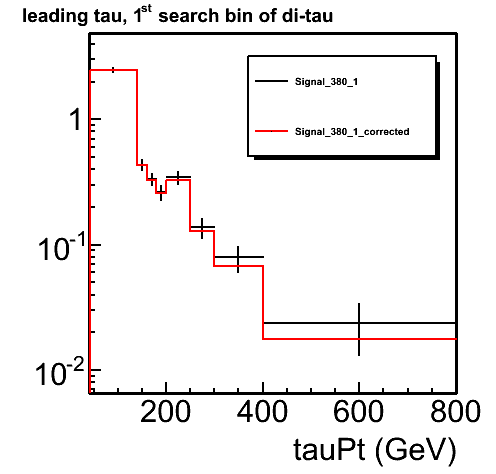
\includegraphics[angle=0,scale=0.35]{TauTauFigs/leadingTauPt.png}
\caption{The $\pt$ distribution of the leading $\hadtau$ in \binone of the $\tauTau$ channel. Also shown is the modified $\pt$ distribution after correction for the trigger bug.}
\label{fig:tauPt}
\end{figure}

 The choice of this signal point is because of the fact that this SMS point can provide the maximum efficiency of 
having $\hadtau$ with $\pt$s above 140 \GeV.  In the same plot, the modified pt-distribution is shown in red, 
which is obtained as follows. Based on figure~35 of the same reference, a correction factor is taken and 
multiplied bin-by-bin to the black histogram (for the bins above 140 GeV). The difference in integral
 of the two histograms is of the order of ~1.5\% (original integral equals 4.10, while the modified integral is equal to 4.04).

\subsection{b-jet ID}
The uncertainty due to the b-tag scale factor on the signal and background events is taken into account by varying the scale factors within their 
uncertainty. It is found that for signal, there is an uncertainty of about $8\%$. For almost all of the backgrounds except for backgrounds including Top, an uncertainty around 1\% is found. For Top backgrounds, the uncertainty is about 4\%. Therefor, for background events at most a 4\% uncertainty due to the b-veto cut is assigned. 
 
\subsection{Lepton trigger, identification and isolation efficiency}
The uncertainties on electron and muon triggers, identification and isolation efficiencies are $2\%$ for electrons and muons ~\cite{CMS_AN_2013-171}. The uncertainty on the $\hadtau$ identification efficiency amounts to $6\%$ ~\cite{CMS_AN_2013-171}
The uncertainty on the efficiency of the hadronic tau leg of the $e\hadtau$ and $\mu\hadtau$ ($\tauTau$) trigger amounts to $3.0\%$ ($4.5\%$ per leg).

\subsection{PDF}
The signal acceptance changes due to PDF uncertainties is expected to be small. We take this uncertainty from ~\cite{CMS_AN_2012-248}, where the signal has been produced through electroweak process like our signal. The amount of this uncertainty is around $2\%$.
The effect of PDF on cross section is considered using $CTEQ66$ and $MSTW2008nlo90cl$ for PDF and it is shown for some generic SUSY points in Table.~\ref{Tab.PDF}.
% We also looked at the other searches like ``CMS AN-14-120'', edge analysis, where the PDF uncertainties on the signal acceptance are evaluated to vary between 1% and 5%.


\begin{table}[!h]
\begin{center}
\begin{tabular}{|c|c|c|}
\hline
                                    &$\sigma (fb) \_ CTEQ66$          & $\frac{\sigma \_ CTEQ66 - \sigma \_ MSTW2008}{\sigma \_ CTEQ66}$  \\\hline 
m(\chione) = 100 GeV                &$5823.40^{+0.0 \% + 3.4 \%}_{-0.6 \% - 3.2 \%}$         & 3 \%         \\\hline   
m(\chione) = 200 GeV                &$379.24^{+0.4 \% + 4.5 \%}_{-0.4 \% - 4.4 \%}$          & 6 \%        \\\hline  
m(\chione) = 300 GeV                &$67.51^{+0.2 \% + 5.9 \%}_{-0.2 \% - 5.1 \%}$           & 7 \%        \\\hline
m(\chione) = 400 GeV                &$17.51.40^{+0.0 \% + 6.8 \%}_{-0.3 \% - 6.3 \%}$        & 8 \%        \\\hline
m(\chione) = 500 GeV                &$5.53^{+0.0 \% + 8.1 \%}_{-0.9 \% - 7.0 \%}$            & 12 \%        \\\hline
\end{tabular} 
\end{center}
\caption{Cross section systematic uncertainty due to different PDF.}
\label{Tab.PDF}
\end{table}     
\subsection{Pile-up}

The minimum bias cross section is varied $5 \%$ up and down following the standard recipe of ~\cite{PU_SYS}. It is found to introduce $~4 \%$ systematic for all channels.    

\subsection{\texorpdfstring{$\met$}{met}}

The main backgrounds come from data driven or MC validated against data. \MET uncertainties can be important for signal only. Our signal is produced through an SUSY EWK production and does not include jets directly but it is expected to feature four invisible particles as genuine missing energy. Therefore it should not be affected by jet calibrations. Apart from jets, lepton and tau energy scales and their effects on \MET have been already taken into account. There is just unclustered energy left which based on results in ~\cite{CMS_AN_2014-099} this item's effect on \MET is small enough to be ignored.

\subsection{Low rate backgrounds} For some backgrounds like \ttbar, dibosons and Higgs decays, the remaining 
events from the simulation are very small. A 50\% uncertainty is considered for these backgrounds to account for the theoretical uncertainty of the
cross section calculation as well as the shape mismodeling.

\subsection{Summary}
The summary of all systematic uncertainties for different channels is reported in Table.~\ref{Tab.SYS}. The main source of the systematic uncertainty in all channels and samples is the \hadtau energy scale.

\begin{table}[!h]
\begin{center}
\small{
\begin{tabular}{|l|c|c|c|c|}
\hline\hline
Systematic uncertainty source & \eTau & \muTau & \tauTau SR1 & \tauTau SR2\\
\hline\hline
{Luminosity}&\multicolumn{4}{c|}{$2.6\%$} \\\hline
{$\tau_{had}$ energy scale}&\multicolumn{4}{c|}{$25\%$} \\\hline
{Electron trigger, id, iso efficiency}& $2\%$ & \multicolumn{3}{c|}{} \\\hline
{Muon trigger, id, iso efficiency}& &$2\%$ & \multicolumn{2}{c|}{} \\\hline
{$\tau_{had}$ id efficiency}& \multicolumn{4}{c|}{$6\%$} \\\hline
{$\tau_{had}$ trigger efficiency}& \multicolumn{2}{c|}{$3\%$}&\multicolumn{2}{c|}{$4.5\%$ per leg} \\\hline
{Pile-up}&\multicolumn{4}{c|}{$4\%$} \\\hline
{\MET}&\multicolumn{4}{c|}{$5\%$} \\\hline
{b-jet ID}& $4\%$ & $4\%$ & - & $4\%$ \\\hline
Total(backgrounds) & $26\%$ & $26\%$ & $27\%$  & $27\%$\\\hline
Low rate backgrounds &50\%  & 50\%   & 50\%    & 50\%\\\hline
\multicolumn{5}{|c|}{only for signal} \\\hline
{ISR}&\multicolumn{4}{c|}{$3\%$} \\\hline
{$\mindphifour$}&\multicolumn{4}{c|}{$6\%$} \\\hline
{$\tau_{had}$ energy scale}&\multicolumn{4}{c|}{$15\%$} \\\hline
{PDF}&\multicolumn{4}{c|}{$2\%$} \\\hline
{b-jet ID}& $8\%$ & $8\%$ & - & $8\%$ \\\hline
Total(Signal) & $20\%$ & $20\%$ & $19\%$  & $20\%$\\
\hline
\hline
\end{tabular}
}
\end{center}
\caption{
  Summary of systematic uncertainties.
}
\label{Tab.SYS}
\end{table}


{\bf Saeid, summary of trigger bug and its effect.}
{\bf Eskandari, Please mention which SMS point you have used for your studies.}
